\documentclass[a4paper]{article}

\usepackage[italian]{babel}
\usepackage[utf8]{inputenc}
\usepackage{amsmath}
\usepackage{graphicx}
\usepackage[colorinlistoftodos]{todonotes}
\usepackage{fullpage}

\title{Analisi delle reti sociali applicata al romanzo Il trono di Spade}

\author{Daniele Baschieri}

\date{\today}

\begin{document}
\maketitle

\begin{abstract}
Your abstract.
\end{abstract}

\section{Introduzione}
L'anaisi delle reti sociali è una moderna metodologia di analisi delle relazioni sociali. Il padre fondatore di questa metodologia è Jacob Levi Moreno, fodatore della sociometria, scienza che si occupa delle relazioni interpersonali.\\
L'analisi delle reti sociali trova applicazione negli ambiti più disparati, in ambito fisico, biochimico, genetico e della computer science.\\
In questa relazione si è applicata la metodologia della analisi delle reti sociali al volume Il trono di spade di George R. R. Martin. Con il principale obiettivo di mettere alla prova la versatilità di questo approccio metodologico, e delle sue potenzialità.\\ 

Con questa modalità di ricerca si supera il precendente apporccio basato su casi ovvero sulle proprietà di ciascun elemento, e si passa ad un approccio connessionista o strutturalista, ovvero basato su collegamenti con altri elmenti.\\
L'approccio strutturalista permette di catturare il ruolo che un certo elemento ricopre all'interno della rete in funzione di come si relaziona agli altri elementi della rete.\\
L'approccio connessionista invece è basato su flussi e relazioni, questi possono virtualmente rappresentare il guadagno relativo a ciascuna connessione permettendo pratiche misure di potere.\\
Con queste premesse l'analisi delle reti sociali appare come uno strumento adatto ad analizzare un romanzo, in cui le fitte trame intessono relazioni sociali tra i personaggi. \\
Vi è però una difficoltà intrinseca nell'analizzare un volume di più di mille pagine, in primo luogo la dimensione del volume che rende obbligatoria una analisi automatica, in secondo luogo l'enrome numero dei personaggi più di un centinaio tra i personaggi rilevanti, infine trovare una misura corretta per rappresentare la rete nel modo più obiettivo possibile, senza quindi sprocare il dato con troppe considerazioni personali.

\section{Obiettivi}

Volendo analizzare il primo volume delle Cronache del ghiaccio e del fuoco utilizzando l'analisi delle reti sociali è stato determinante il saper focalizzare un obiettivo chiaro e univoco su cui orientare le scelte implementative e di ricerca.
Essendo infatti questo metodo mutidisciplinare è possibile ricercare nel testo moltissimi parametri applicando di volta in volta nel modo rigorsoso e corretto differenti tecniche della analisi delle reti sociali. Al fine di costruire una rete quanto più ragionevole e sensibile alla trama del romanzo si è scelto di limitare la ricerca a due domande fondamentali:

\begin{itemize}
\item La divisione in casate riesce a spiegare la rete sociale tra i personaggi?
\item La relazione matrimoniale dei personaggi riesce a spiegarne la rete sociale?
\end{itemize}
Da queste due domande principali si diramano alcune considerazioni, secondarie ma altrettanto importanti:

\begin{itemize}
\item Quali tensionamenti emergono dalle reti sociali così definite?
\item Chi sono i personaggi chiave del romanzo?
\item Analizzando lo sviluppo della vicenda è possibile prevedere i personaggi che verranno uccisi da una congiura? E il loro assassino?
\end{itemize}

\section{Metodologia}

Per poter lavorare su un volume di quasi 1000 pagine è stato necessario definire con estrema cura il metodo di indagine.\\
Si è quindi pensato di considerare i personaggi principali del volume tralasciando solo le comparse, prendendo in esame quindi un elenco con i 105 personaggi più importanti tra quelli riportati nelle appendici di fine libro. Per ciascuno di questi personaggi è stato individuato il nome, il titolo e qualsiasi riferimento nel testo che li caratterizzi in modo univoco.\\
\newtheorem{xxx}{Esempio}
Ad esempio Eddard Stark viene elencato come:
\begin{xxx}
Eddard Stark, Eddard, Ned, lord di Grande Inverno, protettore del Nord, lord Stark
\end{xxx}

Definiti gli attori di questa rete è stato necessario calcolare i legami tra questi attori. Si è perciò deciso di dare una nuova definizione di evento ovvero i capitoli, gli attori si incontrano in questi eventi. Il volume è composto da 73 capitoli nei quali si alternano le vicende di questi personaggi, ciascun capitolo è strutturato dal punto di vista di uno specifico personaggio, perciò alcune considerazioni dovranno essere fatte al termine del lavoro.\\
Nel volume troviamo i punti di vista di otto personaggi ovvero: Bran, Catelyn, Daenerys, Eddard, Jon, Arya, Tyrion, Sansa.\\
Per poter popolare la rete sociale si è perciò andato a contare all'interno dei 73 capitoli quante volte ciascuno dei 105 personaggi viene citato.\\
Non è perciò possibile verificare se un personaggio comparendo in un dato capitolo sia davvero presente nel suddetto o venga invece citato in un dialogo da uno degli altri personaggi presenti, quello che però traspare è che quel personaggio anche solo per il fatto di venire menzionato ha una influenza in quello specifico capitolo.\\

Da questo conteggio si è ottenuta una rete bimodale personaggi/capitoli, grazie a questa rete è stato possibile affiliarla in una rete monomodale personaggi/personaggi. Una rete in cui si può valutare le interazioni che ha ciascun personaggio con ogni altro personaggi. Si è ipotizzato che in ciascun capitolo ogni personaggio si relazioni con ogni altro personaggio citato in quel medesimo capitolo. A giustificare questo assunto bisogna tenere presente che l'unità fondamentale è il capitolo e che ciascun capitolo copre uno spettro di 13 pagine, in media, ed essendo i capitoli centrati su un personaggio il ritenere che ogni personaggi in un capitolo tesse le sue relazioni con ogni altro personaggio del capitolo è del tutto ragionevole.\\ 
Più un personaggio appare all'interno di un capitolo più è forte il legame relazionale che tesse con gli altri attori nel medesimo capitolo.



\section{Strumenti}
Fatta ora una premessa sulle scelte implementative bisogna considerare gli sturmenti utilizzati per portare a termine l'analisi.\\

\subsection{Python}
Si è scelto per poter elaborare rapidamente il volume di implementare uno script in pyhton che riesca ad estrapolare dal testo le occorrenze di ciascun personaggio, l'inizio di ciascun capitolo e compattare i risultati ottenuti in un unico file\\
Il lavoro è stato svolto in parallelo applicando il pattern della map-reduce.


\subsection{UciNet}
Per poter elaborare i nodi così ottenuti nella forma: personaggio, capitolo, occorrenze si è utilizzato UciNet\cite{UciNet} un software scritto da Lin Freeman sulla fine degli anni '80 che ha subito numerosi aggiornamenti ed è tutt'ora tra i più utilizzati nello studio delle reti sociali, questo per via della sua interfaccia pratica e intuitiva e per la sua capacità di restituire rapidamente risultati apprezzabili e comparabili.

\section{Analisi}

Analizzando il numero di personaggi e contando globalmente il numero di volte in cui ciascuno di essi viene citato si è potuta produrre una curva che interpoli la frequenza di ciascun personaggio nel romanzo.(Fig. \ref{fig:frequenza-personaggi})

\begin{figure}[h]
\centering
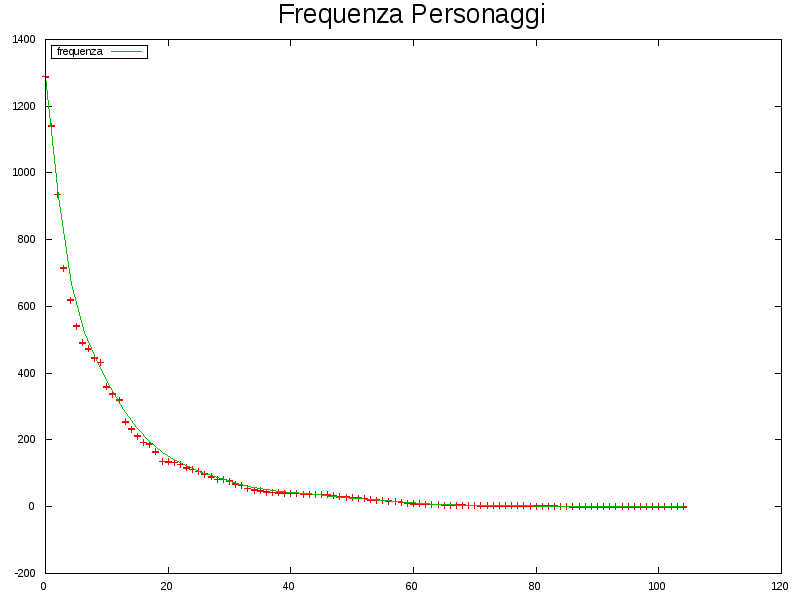
\includegraphics[width=.8\textwidth]{picture/frequenza_personaggi.png}
\caption{Grafico frequenza di ciascun personaggio nel romanzo}
\label{fig:frequenza-personaggi}
\end{figure}

La suddetta distribuzione segue una legge di potenza, ciò suggerisce una cricca di pochi personaggi determinanti e una rete più ampia di personaggi meno importanti. Questa configurazione segue il principio di Pareto, ovvero il 20\% dei personaggi appare più dell'80\% delle volte nel romanzo.\\
Per poter individuare univocamente questo sottoinsieme si è calcolato come segue 
\begin{align}
\sum\limits_{i=1}^n f(personaggio_i ) = 11743\\
x:11743=80:100\nonumber\\
x=11743*80/100\nonumber\\
x=9394,4\nonumber  
\end{align}

Risolta questa equazione otteniamo x che rappresenta l'80\% dei legami della rete, questi legami sono distribuiti su di un numero esiguo di personaggi per poterli individuare si sono trovati tutti quei personaggi per cui la loro somma desse 9394,4.
Tali personaggi appaiono nel romanzo con una frequenza superiore a 165, si è deciso di estendere a 135 includendo nell'insieme Lysa Tully poichè personaggio importante per la vicenda, ciò è corretto essendo la suddivisione 80/20 una scelta empirica è necessario contestualizzarla quanto più possibile per rappresentare il caso reale.\\

Fatto ciò si è poi individuato l'insieme delle triplette:
\newtheorem{triplette}{Esempio}
\begin{xxx}
nodo evento [valore]
\end{xxx}
definita come:
\newtheorem{triplette_es}{Esempio}
\begin{xxx}
personaggio capitolo citazione
\end{xxx}
l'enlenco è stato importato in UciNet come NodeAttr.\\

Sfruttando le funzionalità di UciNet si è affiliato da una bimodale ad una monomodale sulle righe personaggi, scegliendo come modalita la somma dei minimi, (Sums of cross-minimum), ovvero la somma deil valore di legame minimo degli attori rispetto agli eventi. Che è l'equivalente di dire i casi in cui vi è co-orrorrenza.\\ 
Questo al fine di poter esprimere che la co-occorrenza di due personaggi nel medesimo capitolo è influenzata come il minimo della partecipazione tra i due, poichè la relazione tra i due è influenzata dal personaggio meno presente nel capitolo.

A questo grafo si è applicato un filtro rimuovendo tutti i legami di intensità inferiore a 120, si è così rimosso dalla rete tutti quei collegamenti troppo esili per significare davvero un legame tra due personaggi. 

\begin{figure}[h]
\centering
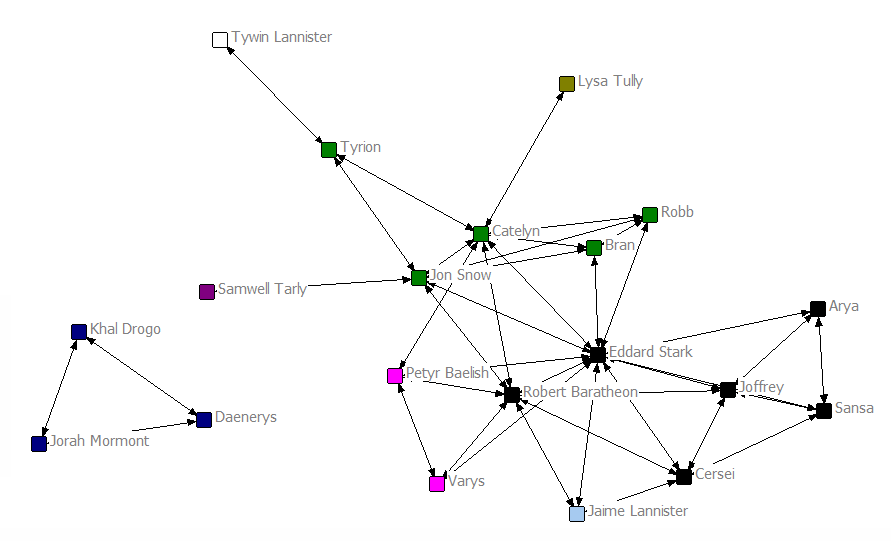
\includegraphics[width=.9\textwidth]{picture/031.png}
\caption{Il Grafo delle reti sociali}
\label{fig:grafo-partito}
\end{figure}
La rete presente in figura uno è stata colorata applicando il metodo di partizione di clique.\\

\subsection{Casate}
Avvalendosi della rete precedentemente ottenuta si è applicato il filtro per sottogruppi, detto clique, ovvero la ricerca dei sottografi completi massimali. In altre parole, si tratta di un sotto-insieme di nodi in cui ogni possibile coppia di punti è direttamente collegata da una linea. Il concetto di clique in italiano cricca è facile da traslittere a casata, infatti laddove saranno presenti delle clique di nodi ci si può aspettare di individuare una casata dove i membri massimizzano le interazioni gli uni con gli altri, gruppi chiusi e resistenti.

Applicando perciò tale raggruppamento si è riuscito ad individuare quelle che a prima vista possono apparire come le casate presenti nel Trono di Spade.\\

Si è quindi scelto di analizzare numericamente quanto questa suddivisione riesca a catturare le reali casate del romanzo.
\begin{itemize}
  \item \emph{Stark:} Eddard, Sansa, Arya, Bran, Robb, Rickon, Lyanna.
  \item \emph{Baratheon:} Robert, Renly, Stannis, Joffrey, Myrcella, Tommen.
  \item \emph{Lannister:} Tywin, Kevan, Cersei, Tyrion, Jaime.
  \item \emph{Tully:} Catelyn, Lysa, Hoster, Bryden.
  \item \emph{Targaryen:} Denerys, Viserys, Aerys, Rhaegar, (Jorah, Drogo).
  \item \emph{Clegane:} Gregor, Sandor.
  \item \emph{Guardiani della Notte:} Jon Snow, Samwell Tarly, Meastro Aemon, Donal Noye, Jeor Mormont.
\end{itemize}

Alcuini di questi personaggi a causa dei filtri precedentemente imposti non compaiono mentre altri risultano collocati in casate differenti rispetto a quelle di origine.

Per poter valutare la correttezza della suddivisione così ottenuta si è rappresentata sotto forma di matrice la  disposizione così individuata.
\\
\begin{tabular}{ c c c c c c c c}
 casate & stark & lannister &  baratheon & targryen & arryn & night-watch & out\\
 stark     & 3 & 0 & 3 & 0 & 0 & 0 & 0\\
 lannister & 1 & 1 & 1 & 0 & 0 & 0 & 1\\
 baratheon & 0 & 0 & 2 & 0 & 0 & 0 & 0\\
 targaryen  & 0 & 0 & 0 & 3 & 0 & 0 & 0\\
 arryn     & 0 & 0 & 0 & 0 & 1 & 0 & 0\\
 niht-watch& 0 & 0 & 0 & 0 & 0 & 1 & 0\\
 out       & 0 & 0 & 2 & 0 & 0 & 0 & 0\\
\end{tabular}
\\
\\
Applicando la formula di chi-quadro sulla matrice così ottenuta siamo in grado di calcolare lo scostmento del risultato rispetto al caso random.\\
Il calcolo del chi quadro ci fornisce la probabilità p = 0.000675369, più è piccola la probabilità più è precisa la divisione così ottenuta. Avendo un valore \begin{math}6*10^{-4}\end{math} si può ragionevolmente supporre di aver ottenuto una divisione piuttosto precisa grazie ai dati forniti in input.

Alla luce di questa partizione bisogna valutare le incongruenze che emergono, sono giustificate?

Vi è una forte confusione tra gli Stark e i Lannister e i Baratheon, questo per via del fatto che questi personaggi si trasferiscono tutti ad Approdo del Re nel corso del romanzo e vivono una fitta trama ricca di alleanze e inimicizie sotterfugi e tradimenti.
Tyrion sebbene unico collegamento con Tywin risulta però non appartenente alla cricca dei Lannister questo poichè viene rapito dagli Stark per una gran parte del romanzo.
Catelyn Tully sebbene sia collegata con Lysa risulta essere una Stark essendo moglie di Eddard Stark.
Eddard invece risulta collegato a Robert Baratheon poichè viene nominato primo cavaliere nelle prime pagine del romanzo e sarà costretto a servire il suo amico e Re durante tutto il volume.


\subsubsection{Allargare lo spettro di indagine}

Al fine di includere un maggior numero di personaggi nella analisi, si è rilassato il vincolo della dicotomizzazione a 135 connessioni, si sono perciò considerati tutti i personaggi del romanzo, e su questi personaggi si è imposto un filtro a 20 connessioni come somma dei minimi incrociati.

La rete che ne consegue è una rete molto più ricca, questa rete risulta essere molto interessante poichè mette in evidenza un numero di relazioni qualitativamente su.

Emerge che Jon Arryn è legato a Lysa Tully e ciò è ragionevole visto il loro legame matrimoniale, si può dire la medesima cosa di Kahal Drogo marito di Daenerys Targaryen.

Stannis e Renly Baratheon invece risultano ben divisi e ciò sarà ulteriormente evidente nei prossimi romanzi dove Stannis finrà per uccidere suo fratello Renly.

I guardiani della notte risultano un insieme non omogeneo giò è dovuto in parte anche al fatto che Benjen Stark sarà dato per disperso nelle prime pagine del libro e che Donal Noye ha un forte legame con Jon Snow.


\subsection{Relazioni Matrimoniali}

Si sono prese in considerazione le seguenti coppie:

\begin{itemize}
\item Khal Drogo - Daenerys Targaryen
\item Robert Baratheon - Cersei Lannister
\item Eddard Stark - Catelyn Tully
\item Jon Arryn - Lysa Tully
\end{itemize}

Ciascuno di questi legami matrimoniali è presente nella rete dicotomizzata a 20.\\
Per poter cogliere eventuali difficotà matrimoniali abbiamo dicotomizzato la rete a 48 e ci siamo accorti che il legame tra Jon Arryn e Lysa Tully si spezza come in Figura \ref{fig:grafo-partito-1500}.\\
\begin{figure}[h]
\centering
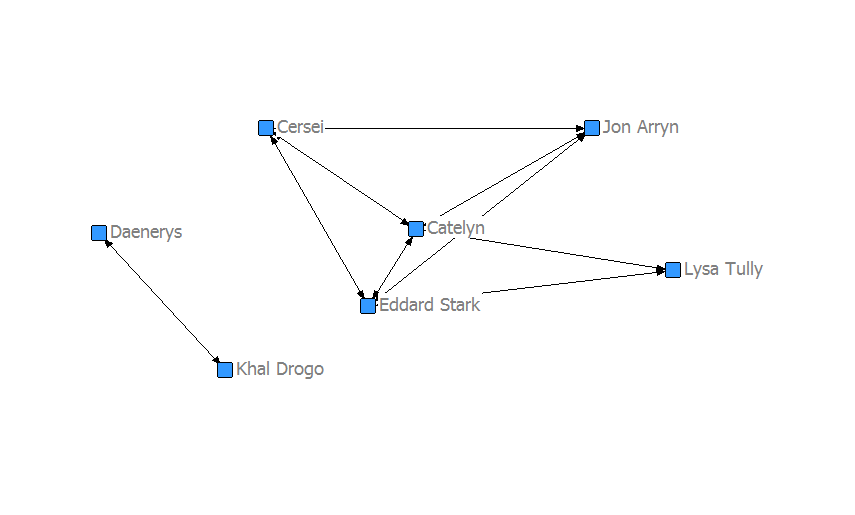
\includegraphics[width=.9\textwidth]{picture/32.png}
\caption{La componente principale del grafo dicotomizzato a 1500}
\label{fig:grafo-partito-1500}
\end{figure}
Per poter rompere altri legami matrimoniali bisogna spingersi a 227 dove si spezza il legame tra Robert Baratheon e Cersei Lannister.

Possiamo quindi dire la forza del legame di coppia è come segue, l'amore più forte lega i Tully agli Stark, seguiti da i Targaryen con i Khal, a seguire i Baratheon con i Lannister e per finire un labile legame tra gli Arryn e i Tully.

Questo è piuttosto evidente nella lettura del romanzo, dove infatti, la rottura di queste relazioni matrimoniali causeranno importani sviluppi nella vicenda.


\subsection{La morte del re}
L'evento centrale del primo romanzo è indubbiamente l'assassinio di Robert Baratheon il re dei sette regni.
Per poter individuare il suo assassino si è pensato di effettuare una ricerca nella sua rete sociale.\\
Per avere una rete più sensibile alle duplici relazioni di ciascun personaggio si è deciso di affiliare la rete personaggi capitoli in una monomodale personaggi personatti come somma dei prodotti incrociati.\\ 
Alla rete così prodotta si è applicata una dicotomizzazione di tutti quei collegamenti superirori a 50, ovvero il cuoi prdotto rispetto ad un dato capitolo fosse superiore almeno a cinquanta, e si è scartato il resto.\\
Si è deciso di dicotomizzare per rimuovere le occorrenze casuali tra i personaggi in modo da avere solo riferimenti reali.\\
Per poter individuare un colpevole si è decisa come metrica di indagine la ricerca dei buchi strutturali presenti nella rete.
Buco strutturale o detto \textit{Structural hole} è un termine coniato da Ronald Burt, per indicare la particolare e favorevole posizione di un nodo rispetto ai suoi vicini. Se A B C sono collegati tutti insieme non sono presenti buchi strutturali mentre se A-B e B-C sono collegati è presente un buco strutturale tra A-C, questo collegamento mancante porta un discreto vantaggio al nodo B.
Esistono diverse misure di buco strutturale in questo articolo ci si è concentrati sulla \textit{Dyadic constraint}.
Dyadic constraint è una misura che rappresenta un indice di quanto i vicini di \textit{Ego} influenzino il nodo.
Si è perciò scelto come nodo Robert Baratheon e si è analizzato come i suoi vicini lo influenzino.
Nella figura \ref{fig:grafo-dyadic-constraint} è stato evidenziato in rosso il nodo centrale, e in arancione i nodi con la più alta Dyadic Constraint, da qui si possono fare qualcune valutazioni sui risultati.
\begin{itemize}
\item \textbf{Jalabhar Xho} mercante di spezie che abita in una terra lontana.
\item \textbf{Preston Greenfield} uno delle fedelissime spade giurate del Re.
\item \textbf{Rhaenys Targaryen} una principessa Targaryen che è però ormai morta da anni al epoca dei fatti.
\item \textbf{Lancel Lannister} scudiero di Re Robert la cui fedeltà va però ai Lannister.
\item \textbf{Robert Arrynr} principe di Nido Dell'Acquila figlio del miglior amico di Robert, ragazzo malaticcio e malfermo, non ha mai abbandonato casa propria.
\end{itemize}

\begin{figure}[h]
\centering
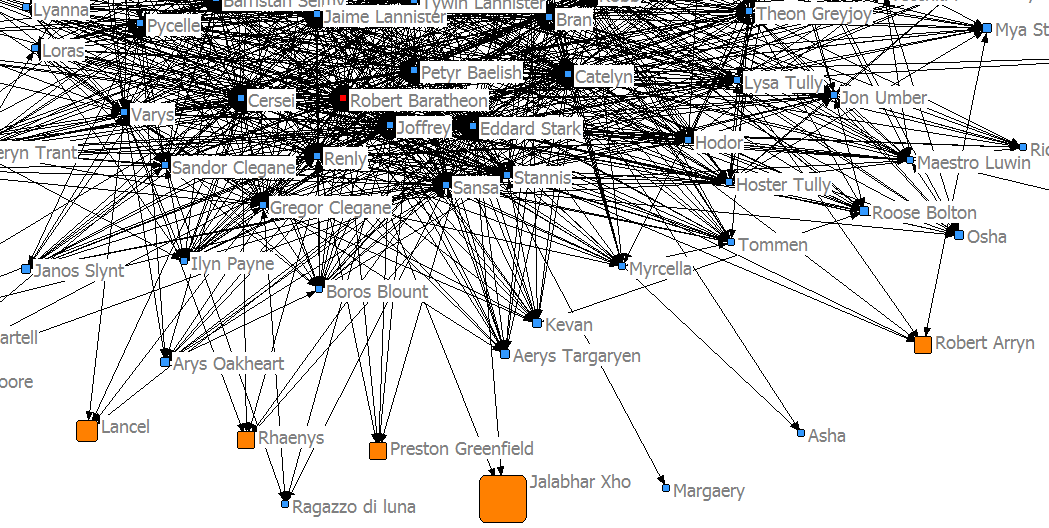
\includegraphics[width=.8\textwidth]{picture/33.png}
\caption{Grafo relativo alla rete con applicato il filtro Dyadic constraint}
\label{fig:grafo-dyadic-constraint}
\end{figure}

Il più apettibile tra i personaggi è sicuramente Lancel Lannister coppiere personale del re, fedele alla casata dei Lannister di cui fa parte la moglie del Re, Cersei, la quale sappiamo avere un basso legame affettivo con il marito dalla precedente analisi.\\
Essendo quindi tra i presenti l'unico personaggio dotato di un movente e della effettiva possibilità di compiere il gesto si può ritenere che sia il più probabile colpevole del delitto.\\
La lettura del romanzo supporta infatti questo risultato.

\subsection{potere, influenza e cambiamento}

Si è poi deciso di suddividere il romanzo in tre porzioni in ordine cronologico, collegando i capitoli dal 1 al 25 dal 26 al 50 e dal 51 al 73, questo al fine di comprendere eventuali variazioni di influenza tra i personaggi.

Per poter valutare l'influenza di ciascun personaggio ci si è affidati al calcolo della betweenness, ovvero della centralità del nodo rispetto a tutti i cammini più brevi tra ogni altra coppia di nodi. Infatti più un nodo è al centro dei cammini minimi tra ogni altra coppia di nodi, più l'esistenza di questo nodo è essenziale al passiaggio di informazioni attraverso la rete.

I nodi che subiscono una maggiore variazione nella betweenness nelle tre fasi del romanzo sono:
Arya Stark, Sansa Stark, Joffrey Baratheon, Petyr Baelish, Varys, Tywin Lannister, Jamie Lannister, Stannis Baratheon, Daenerys Targaryen e Jorah Mormont.

Nella fase centrale del romanzo c'è infatti un leggero ribaltamento degli equilibri che porta molto vantaggio ai Lannister, tra cui spiccano Tywin Jamie e Joffrey (figlio di Cersei e di fatto un Lannister), che chiuderanno il romanzo vedendo raddoppiare la loro centralità.
Daenerys e Jorah Mormont accresceranno la loro betweenness nelle fasi centrali del romanzo, è infatti questo il momento in cui le lettere traditrici di Jorah Mormont raggiungono il concilio ristretto di Robert Baratheon portando notizie su Daenerys. (Capitolo 33)
Altri due personaggi minori che acquisiscono molto potere sono Petyr Baelish e Varys, il cui ruolo di comparsa iniziale si trasforma progressivamente in ruolo chiave per le sorti del regno.
Altro personaggio non marginale ad accrescere la propria influenza è Stannis che alla morte di Robert si autoproclamerà suo successore.



\section{Conclusioni}


\begin{thebibliography}{9}
  \bibitem{UciNet}
  	Borgatti, S.P., Everett, M.G. and Freeman, L.C. 2002. 		\emph{Ucinet for Windows: Software for Social Network Analysis. Harvard, MA: Analytic Technologies.} 
\end{thebibliography}

\end{document}